\documentclass[margin=5mm]{standalone}
\usepackage[dvipsnames]{xcolor}
\usepackage{pgfplots}
\usepackage{tikz}
\usepackage[tikz]{ocgx2}

\pgfplotsset{compat=1.18}
\begin{document}

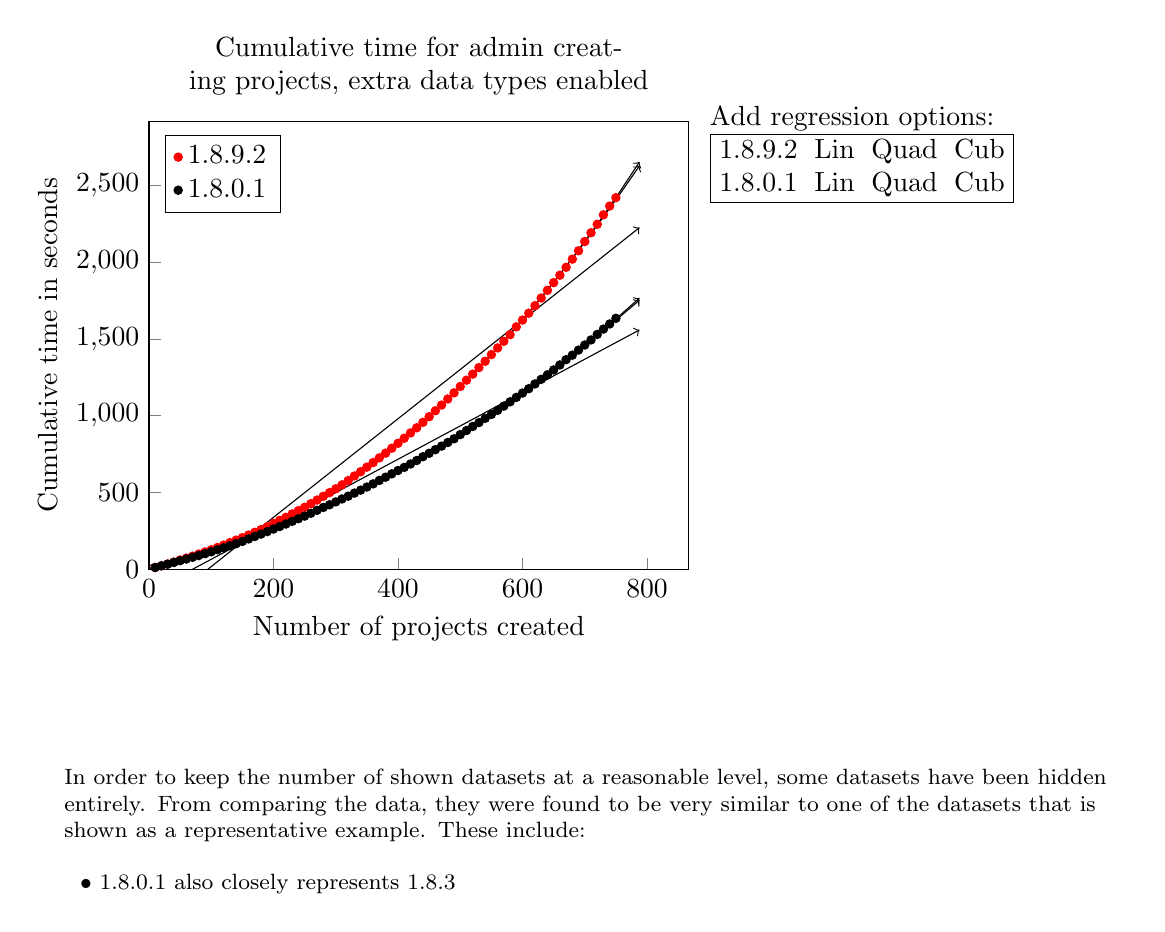
\begin{tikzpicture}
    \begin{axis}[
        align = center,
        legend pos = north west,
        legend cell align = left,
        xlabel = Number of projects created,
        ylabel = Cumulative time in seconds,
        xtick pos = left,
        ytick pos = left,
        scaled ticks = false,
        xmin = 0,
        ymin = 0,
        title = {Cumulative time for admin creating projects, extra data types enabled},
        title style = {text width = 0.8\textwidth},
        legend entries={\switchocg{1.8.9.2}{1.8.9.2},\switchocg{1.8.0.1}{1.8.0.1}}]
        \begin{scope}[ocg = {ref = 1.8.9.2-Lin, status = invisible}]
            \plot[domain=0:788,->,forget plot] (\x,{-302.4888018018021966781816445291042327880859375 + 3.207316460881935338278481140150688588619232177734375*(\x)^1});
        \end{scope}
        \begin{scope}[ocg = {ref = 1.8.9.2-Quad, status = invisible}]
            \plot[domain=0:788,->,forget plot] (\x,{25.648580303590506446198560297489166259765625 + 0.6504017951256282348282411476247943937778472900390625*(\x)^1 + 0.0033643614023109312712034313364029003423638641834259033203125*(\x)^2});
        \end{scope}
        \begin{scope}[ocg = {ref = 1.8.9.2-Cub, status = invisible}]
            \plot[domain=0:788,->,forget plot] (\x,{8.4864582409796565087845010566525161266326904296875 + 0.9127349839877492154727178785833530128002166748046875*(\x)^1 + 0.0025071125480346655341190587051869442802853882312774658203125*(\x)^2 + 0.0000007519726791897069581802341871334949274796599638648331165313720703125*(\x)^3});
        \end{scope}
        \begin{scope}[ocg = {ref = 1.8.9.2, status = visible}]
            \addplot[
                only marks,
                color = red,
                mark = *,
                mark size = 1.5 pt
            ]coordinates {(10,12.529)(20,23.575)(30,34.966)(40,47.945)(50,61.027)(60,73.597)(70,86.304)(80,100.058)(90,113.519)(100,127.803)(110,142.754)(120,158.14)(130,174.614)(140,190.779)(150,206.634)(160,223.645)(170,241.54)(180,258.97)(190,277.386)(200,299.75)(210,319.359)(220,339.151)(230,361.127)(240,382.525)(250,404.09)(260,427.475)(270,451.39)(280,475.926)(290,499.478)(300,524.561)(310,550.292)(320,578.285)(330,608.041)(340,635.811)(350,665.656)(360,695.249)(370,725.814)(380,756.507)(390,788.475)(400,820.626)(410,853.585)(420,888.115)(430,921.523)(440,957.177)(450,993.914)(460,1032.533)(470,1069.651)(480,1109.18)(490,1148.924)(500,1190.345)(510,1231.427)(520,1270.955)(530,1313.464)(540,1354.681)(550,1398.032)(560,1441.346)(570,1484.662)(580,1527.329)(590,1578.367)(600,1622.978)(610,1667.354)(620,1716.09)(630,1766.171)(640,1816.143)(650,1866.284)(660,1914.545)(670,1966.018)(680,2019.196)(690,2073.937)(700,2133.84)(710,2190.838)(720,2246.121)(730,2307.717)(740,2364.717)(750,2419.327)};
        \end{scope}
        \begin{scope}[ocg = {ref = 1.8.0.1-Lin, status = invisible}]
            \plot[domain=0:788,->,forget plot] (\x,{-151.165728288288420344542828388512134552001953125 + 2.170149004267425407732616804423741996288299560546875*(\x)^1});
        \end{scope}
        \begin{scope}[ocg = {ref = 1.8.0.1-Quad, status = invisible}]
            \plot[domain=0:788,->,forget plot] (\x,{6.86647521658613602113518936675973236560821533203125 + 0.93872923669697438953107848647050559520721435546875*(\x)^1 + 0.0016202891678558568357149116678783684619702398777008056640625*(\x)^2});
        \end{scope}
        \begin{scope}[ocg = {ref = 1.8.0.1-Cub, status = invisible}]
            \plot[domain=0:788,->,forget plot] (\x,{-2.64790004771925424620349076576530933380126953125 + 1.084162091329429866704003870836459100246429443359375*(\x)^1 + 0.00114504564816027862121650127136263108695857226848602294921875*(\x)^2 + 0.0000004168802804347179760953803241696480341715869144536554813385009765625*(\x)^3});
        \end{scope}
        \begin{scope}[ocg = {ref = 1.8.0.1, status = visible}]
            \addplot[
                only marks,
                color = black,
                mark = *,
                mark size = 1.5 pt
            ]coordinates {(10,12.528)(20,23.237)(30,34.244)(40,45.411)(50,56.703)(60,67.523)(70,78.658)(80,90.17)(90,102.073)(100,114.874)(110,128.109)(120,140.539)(130,154.004)(140,167.615)(150,182.124)(160,198.157)(170,214.455)(180,229.863)(190,245.902)(200,262.761)(210,279.303)(220,295.501)(230,312.844)(240,329.698)(250,346.84)(260,365.214)(270,384.988)(280,402.918)(290,420.704)(300,439.304)(310,458.319)(320,476.608)(330,496.879)(340,516.104)(350,536.144)(360,556.615)(370,579.251)(380,600.094)(390,622.031)(400,643.569)(410,663.913)(420,685.995)(430,708.734)(440,733.404)(450,755.811)(460,779.135)(470,802.376)(480,825.926)(490,850.052)(500,877.263)(510,903.614)(520,930.306)(530,955.521)(540,983.215)(550,1008.777)(560,1035.233)(570,1062.835)(580,1090.544)(590,1119.381)(600,1147.664)(610,1176.034)(620,1206.946)(630,1237.297)(640,1266.475)(650,1298.156)(660,1330.63)(670,1364.674)(680,1394.284)(690,1427.509)(700,1460.476)(710,1493.333)(720,1529.289)(730,1564.023)(740,1597.156)(750,1633.958)};
        \end{scope}
    \end{axis}
    \begin{scope}
        \addtolength{\tabcolsep}{-0.3em}
        \node [below right, shape=rectangle, align=left](regressiontable) at (7,6) {
            Add regression options: \\
            \begin{tabular}{|llll|}
                \hline
                1.8.9.2 & \switchocg{1.8.9.2-Lin}{Lin} & \switchocg{1.8.9.2-Quad}{Quad} & \switchocg{1.8.9.2-Cub}{Cub} \\
                1.8.0.1 & \switchocg{1.8.0.1-Lin}{Lin} & \switchocg{1.8.0.1-Quad}{Quad} & \switchocg{1.8.0.1-Cub}{Cub} \\
                \hline
            \end{tabular}
        };
    \end{scope}
    \begin{scope}[every node/.style = {font=\footnotesize}, right]
        \node[text width = 13.5 cm] at (-1.2,-3) {In order to keep the number of shown datasets at a reasonable level, some datasets have been hidden entirely. From comparing the data, they were found to be very similar to one of the datasets that is shown as a representative example. These include:};
        \node at (-1,-4.0) {$\bullet$ 1.8.0.1 also closely represents 1.8.3};
    \end{scope}
\end{tikzpicture}

\end{document}